%%%%%%%% ImpCML 2026 response paper, built on the ICML 2021 template supplied with the coursework %%%%%%%%
\documentclass{article}

\usepackage{microtype}
\usepackage{graphicx}
\usepackage{booktabs}
\usepackage{xcolor}
\usepackage{amsmath,amssymb,amsthm}
\usepackage{hyperref}
\newcommand{\theHalgorithm}{\arabic{algorithm}}

\definecolor{imperialblue}{rgb}{0, 0, 0.804}
\definecolor{springgreen}{rgb}{0, 0.5, 0.5}
\definecolor{violet}{rgb}{0.7803, 0.082, 0.52156}
\newcommand{\csection}[1]{\section{\textcolor{imperialblue}{#1}}}
\newcommand{\csubsection}[1]{\subsection{\textcolor{springgreen}{#1}}}

\usepackage{icml2021}

\theoremstyle{plain}
\newtheorem{proposition}{Proposition}
\newcommand{\R}{\mathbb{R}}
\newcommand{\E}{\mathbb{E}}
\newcommand{\bx}{\mathbf{x}}
\newcommand{\bb}{\mathbf{b}}
\newcommand{\bw}{\mathbf{w}}
\newcommand{\X}{\mathbf{X}}
\newcommand{\W}{\mathbf{W}}
\newcommand{\A}{\mathbf{A}}
\newcommand{\B}{\mathbf{B}}
\newcommand{\G}{\mathbf{G}}
\newcommand{\U}{\mathbf{U}}
\newcommand{\sgn}{\operatorname{sgn}}
\newcommand{\din}{d_{\mathrm{in}}}
\newcommand{\dout}{d_{\mathrm{out}}}
\graphicspath{{figures/}}

% Generated by report/make_numbers.py from results/*.json -- do not edit by hand.
\newcommand{\etaPct}{3.9}
\newcommand{\BayesPct}{96.1}
\newcommand{\LimitTwo}{56.5}
\newcommand{\LimitSix}{95.0}
\newcommand{\LimitSeven}{96.1}
\newcommand{\WeightFourEight}{85}
\newcommand{\MockTwentyTen}{58.4}
\newcommand{\MockThirtyTen}{55.4}
\newcommand{\MockFortyTen}{54.1}
\newcommand{\SelFixedTwenty}{83.0}
\newcommand{\SelFixedThirty}{87.0}
\newcommand{\SelFixedForty}{89.6}
\newcommand{\SelTunedTwenty}{95.6}
\newcommand{\SelTunedThirty}{96.0}
\newcommand{\SelTunedForty}{95.8}
\newcommand{\MLPTwentyMean}{93.8}
\newcommand{\MLPThirtyMean}{94.9}
\newcommand{\MLPFortyMean}{95.3}
\newcommand{\SparseTwentyMean}{95.6}
\newcommand{\SparseThirtyMean}{96.0}
\newcommand{\SparseFortyMean}{95.8}
\newcommand{\TimeKernel}{45}
\newcommand{\TimeSparse}{38}
\newcommand{\TimeMLP}{139}
\newcommand{\MLPconfigs}{$n=20$: depth 3, dropout 0.2; $n=30$: depth 3, dropout 0.2; $n=40$: depth 3, dropout 0.2}
\newcommand{\NmlpTwenty}{5,500}
\newcommand{\NmlpThirty}{7,600}
\newcommand{\NmlpForty}{14,000}
\newcommand{\MLPgrowth}{2.6}
\newcommand{\NsparseTwenty}{2,900}
\newcommand{\NsparseThirty}{2,800}
\newcommand{\NsparseForty}{2,900}
\newcommand{\ZeroShotMean}{50.0}
\newcommand{\LPMean}{50.9}
\newcommand{\MLPProbeMean}{49.9}
\newcommand{\ScratchMean}{52.0}
\newcommand{\FullFTMean}{90.2}
\newcommand{\LoRAoneMean}{95.4}
\newcommand{\SwapMean}{95.6}
\newcommand{\LoRAminMean}{94.8}
\newcommand{\SwapZeroShotPct}{96.0}
\newcommand{\ZeroShotAllPct}{49.5}
\newcommand{\ProbeBitZero}{97}
\newcommand{\ProbeBitNineteen}{58}
\newcommand{\LoRAatFourHundred}{83.3}
\newcommand{\LoRAatEightHundred}{94.7}
\newcommand{\LoRAatSixteenHundred}{93.1}
\newcommand{\FullFTatFourHundred}{55.9}
\newcommand{\FullFTatEightHundred}{63.2}
\newcommand{\FullFTatSixteenHundred}{82.1}
\newcommand{\FullFTatMax}{89.8}
\newcommand{\LoRAaZero}{-0.81}
\newcommand{\LoRAaNineteen}{+0.78}
\newcommand{\LoRAaRest}{0.04}
\newcommand{\LoRAcos}{0.75}
\newcommand{\NetRatio}{0.66}
\newcommand{\StepFull}{5.7}
\newcommand{\StepLoRA}{2.2}
\newcommand{\AgreeTwenty}{97.7}
\newcommand{\AgreeThirty}{99.3}
\newcommand{\AgreeForty}{99.5}
\newcommand{\AgreeSwap}{99.8}
\newcommand{\TotalHours}{4.3}
\newcommand{\TotalWh}{109}
\newcommand{\TotalG}{14}
\newcommand{\TotalGhi}{19}


\icmltitlerunning{\textcolor{violet}{Ten Hidden Bits and a Rank-One Fix: A Response to Kryptonite-3.0}}

\begin{document}

\twocolumn[
\icmltitle{\textcolor{black}{Ten Hidden Bits and a Rank-One Fix: \\ A Response to Kryptonite-3.0}}

\icmlsetsymbol{equal}{*}
\begin{icmlauthorlist}
\icmlauthor{Group Member One}{equal,Imp}
\icmlauthor{Group Member Two}{equal,Imp}
\icmlauthor{Group Member Three}{equal,Imp}
\icmlauthor{Group Member Four}{equal,Imp}
\end{icmlauthorlist}
\icmlaffiliation{Imp}{Department of Computing, Imperial College London, London, United Kingdom}
\icmlcorrespondingauthor{Group Member One}{first.last@imperial.ac.uk}
\icmlkeywords{Machine Learning, Challenge Datasets, Fourier Analysis, LoRA}
\vskip 0.3in
]

\printAffiliationsAndNotice{\icmlEqualContribution}

\begin{abstract}
\citet{quinn2026kryptonite} claim that the Kryptonite-3.0 datasets defeat polynomial basis expansion, more training data and a purpose-built foundation model, KryptoNet-40.
We show that every Kryptonite task is the same Boolean function of only ten of the $n$ input bits, a two-bit parity combined with two four-bit gadgets, observed with \etaPct\% label noise, so the best achievable accuracy is about \BayesPct\%.
This function has almost no low-degree Fourier weight, which explains the mock paper's 55\% results, yet it is a degree-6 polynomial threshold function: the mock paper's own model on ten coordinates selected from training data reaches \SparseFortyMean\% on Kryptonite-40, and an MLP trained from scratch \MLPFortyMean\%.
Learning curves show that more data helps every model that can represent the function, while the quadratic model studied by the mock paper is provably capped at \LimitTwo\%.
Kryptonite-40-Adapt is KryptoNet-40's pretraining task with one input coordinate moved, so LoRA of rank one on the first layer (552 trainable parameters) adapts KryptoNet-40 to \LoRAoneMean\% at two-thirds of the per-step operations of full fine-tuning.
\end{abstract}

%=======================================================================================================
\csection{Introduction}
%=======================================================================================================
Challenge datasets audit claims about machine learning by exposing what current methods cannot do \citep{chollet2019measure}, but only if each failure is attributed correctly: to approximation (no function in the hypothesis class fits), estimation (too few samples to find it) or optimisation (training does not find it). The Kryptonite-3.0 mock paper \citep{quinn2026kryptonite} attributes three failures to machine learning itself: polynomial basis expansion up to degree 10 stays below 59\%, said to contradict universal approximation; quadrupling the data barely helps, so the difficulty is ``intrinsic''; and the foundation model KryptoNet-40 is ``worse than a coin flip'' on Kryptonite-40-Adapt, even when probed.

We treat each claim as a falsifiable hypothesis. We first measure the structure of the data with Fourier analysis on the Boolean hypercube \citep{odonnell2014analysis}, which reveals which coordinates matter and how hard the labels are for polynomials, kernels and networks, and then run controlled experiments that change one factor at a time.

Section~\ref{sec:method} develops the theory, including low-rank adaptation \citep[LoRA;][]{hu2022lora} and its operation count; Section~\ref{sec:design} states four hypotheses and our safeguards; Section~\ref{sec:results} reports the anatomy of the data, polynomial models with and without feature selection, nine learners on five shared splits, learning curves, and the adaptation of KryptoNet-40.

All three claims fail. Every task is one fixed 10-bit Boolean function hidden among $n-10$ distractor bits. Polynomials represent it from degree 6, so universal approximation is not contradicted; the mock paper's models lack samples for their $\binom{n+d}{d}$ features and succeed once irrelevant coordinates are removed. More data helps every model that can represent the function, and KryptoNet-40 needs only a rank-one change to its first layer, which LoRA finds. We expect about 96\% on all four hidden sets and release all code and predictions.\footnote{GitLab repository: \url{https://gitlab.doc.ic.ac.uk/GROUP/kryptonite-response}, commit \texttt{COMMITHASH}.}

\begin{figure*}[t]
\centering
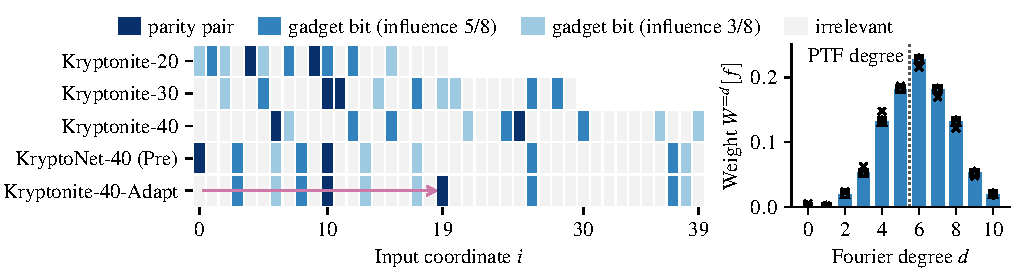
\includegraphics{fig1_anatomy.pdf}
\vskip -0.05in
\caption{Anatomy of Kryptonite-3.0. \emph{Left:} coordinates selected from training data, coloured by their influence on the estimated label function. Every task reads exactly 10 coordinates with the same roles; Adapt is KryptoNet-40's pretraining task with the parity bit at coordinate 0 moved to 19 (arrow). \emph{Right:} Fourier weight of the label function by degree (bars: Kryptonite-40; markers: the other four tasks, which coincide); the function is a polynomial threshold function (PTF) of degree 6.}
\label{fig:anatomy}
\vskip -0.15in
\end{figure*}

%=======================================================================================================
\csection{Methodology}
\label{sec:method}
%=======================================================================================================
\csubsection{Data Model and Fourier Analysis}
We observe $\{(\bx^{(i)},y^{(i)})\}_{i=1}^N$ with $\bx\in\R^n$, $y\in\{0,1\}$, and write $s=2y-1$ and $\bb=\sgn(\bx)\in\{\pm1\}^n$. Every $f:\{\pm1\}^n\to\{\pm1\}$ has a unique multilinear (Fourier) expansion
\begin{equation}
f(\bb)=\sum_{S\subseteq[n]}\hat f(S)\,\chi_S(\bb),\qquad \chi_S(\bb)=\prod_{i\in S}b_i ,
\label{eq:fourier}
\end{equation}
with $\hat f(S)=\E_{\bb}[f(\bb)\chi_S(\bb)]$ under the uniform distribution and $\sum_S\hat f(S)^2=1$. We call $W^{=d}[f]=\sum_{|S|=d}\hat f(S)^2$ the weight at degree $d$, and $\mathrm{Inf}_i[f]=\sum_{S\ni i}\hat f(S)^2$, the probability that flipping $b_i$ flips $f$, the influence of coordinate $i$. With labels flipped at rate $\eta$, sample means of $s\chi_S(\bb)$ estimate $(1-2\eta)\hat f(S)$ with standard error $N^{-1/2}$. By~\eqref{eq:fourier}, a function of $k$ coordinates is \emph{exactly} a polynomial of degree $\le k$ in them.

\begin{figure*}[t]
\centering
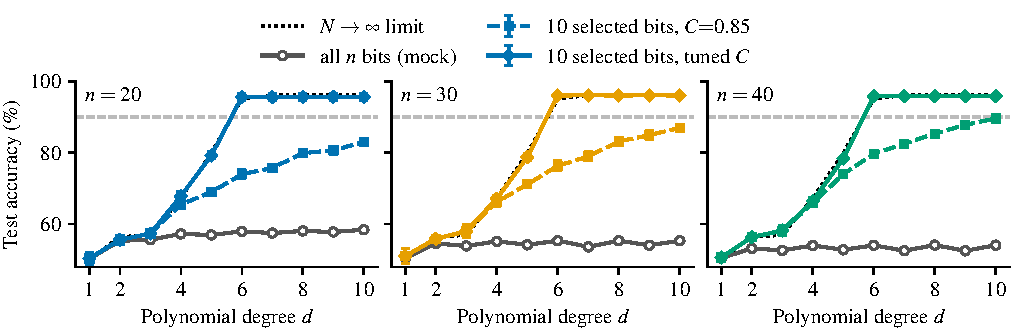
\includegraphics{fig2_polynomial.pdf}
\vskip -0.05in
\caption{Polynomial logistic regression against degree $d$. Grey: the mock paper's model on all $n$ bits, reproduced on its split. Coloured: the same model on the 10 coordinates selected from training data, with the mock paper's $C=0.85$ (dashed) or with $C$ chosen on validation data (solid); mean and 95\% CI over 5 splits. Dotted: infinite-data limit of degree-$d$ logistic regression. Dashed grey: the 90\% target.}
\label{fig:poly}
\vskip -0.15in
\end{figure*}

\csubsection{Polynomial Logistic Regression}
\label{sec:method-poly}
Logistic regression with basis $\phi$ models $P(y=1\mid\bx)=\sigma(\bw^\top\phi(\bx))$ and minimises $C\sum_i\ell(y^{(i)},\bw^\top\phi(\bx^{(i)}))+\frac12\|\bw\|^2$ with the log-loss $\ell$; $C=0.85$ in the mock paper. On $\pm1$ bits every monomial of degree $\le d$ reduces to a parity $\chi_S$ with $|S|\le d$, so the model is a polynomial threshold function (PTF) $\sgn(\sum_{|S|\le d}w_S\chi_S)$. The mock paper fits it in the dual with the normalised kernel $k(\bb,\bb')=\sum_{|S|\le d}c_{|S|}\chi_S(\bb)\chi_S(\bb')/Z$ and Newton's method \citep{rasmussen2006gpml}; on $k$ selected bits we fit the identical model in the primal, with at most $2^k$ features $\sqrt{c_{|S|}/Z}\,\chi_S$.

\begin{proposition}[the quadratic model is capped]
\label{prop:quad}
Let $f=\chi_P\,g$ with $P=\{p,q\}$ and $g$ independent of $b_p,b_q$, and let labels be flipped with rate $\eta$. Over all polynomials of degree $\le2$ in the bits (or in the raw features), the population logistic loss is minimised by $c^\star x_px_q$, whose accuracy is $\frac12\bigl(1+|\hat f(P)|\bigr)(1-2\eta)+\eta$.
\end{proposition}
The proof (Appendix~\ref{app:proofs}) uses a symmetry: negating $x_q$ negates the label, so the unique minimiser can only use monomials of odd degree in both $x_p$ and $x_q$. Logistic regression is consistent for this minimiser, so no amount of data takes the quadratic model beyond it: \LimitTwo\% for Kryptonite.

\csubsection{Kernels, Trees and Neural Networks}
\label{sec:method-learners}
\textbf{Kernels.} The approximation theorems cited by the mock paper \citep{debranges1959stone,hornik1991approximation} are existence statements and say nothing about sample size. For dot-product kernels on the hypercube the parities are eigenfunctions, and with $N\asymp n^{\ell+\delta}$ samples kernel ridge regression learns the projection of the target onto degree-$\le\ell$ polynomials and nothing more \citep{ghorbani2021linearized,mei2022generalization}. Here $N\approx10^4$ and $n\ge20$ give $\log N/\log n<3$, so even a degree-10 kernel effectively fits only the degree-$\le2$ part of $f$. RBF kernels and $k$-NN suffer likewise, as irrelevant coordinates dominate their distances; on the 10 relevant bits, by contrast, the whole function space has dimension $2^{10}\ll N$.

\textbf{Trees.} Random forests \citep{breiman2001random} and gradient boosting split greedily on one coordinate at a time, so when every bit is independent of the label ($W^{=1}[f]=0$) the first splits are uninformative.

\textbf{Neural networks.} An MLP $f_\theta(\bx)=\bw_L^\top\mathrm{ReLU}(\W_{L-1}\cdots\mathrm{ReLU}(\W_1\bx+\mathbf{b}_1))$ is trained on mini-batches $\mathcal B_t$ with AdamW \citep{kingma2015adam,loshchilov2019decoupled}: with $\mathbf g_t=\nabla_\theta\frac1{|\mathcal B_t|}\sum_{i\in\mathcal B_t}\ell(y^{(i)},f_\theta(\bx^{(i)}))$ and bias-corrected moment estimates $\hat{\mathbf m}_t,\hat{\mathbf v}_t$ of $\mathbf g_t$ and $\mathbf g_t^2$,
\begin{equation}
\theta_{t+1}=\theta_t-\alpha\bigl(\hat{\mathbf m}_t/(\sqrt{\hat{\mathbf v}_t}+\epsilon)+\lambda\theta_t\bigr),
\label{eq:adam}
\end{equation}
with learning rate $\alpha$, weight decay $\lambda$, batch size $|\mathcal B_t|$ and the number of epochs (set by early stopping) as hyper-parameters. Unlike a kernel, the network can align its first layer with the relevant coordinates. For two-layer networks trained by SGD, the sample complexity of a sparse function is governed by its \emph{leap}, the largest number of new coordinates that must be found at once along its Fourier support, and scales as $\tilde O(n^{\max(\mathrm{Leap}-1,1)})$ \citep{abbe2022merged,abbe2023leap}. Kryptonite has leap 2 (Section~\ref{sec:anatomy}): polynomial in $n$ with an exponent that does not grow with the degree, unlike the $\binom{n+6}{6}$ features of a degree-6 kernel.


\begin{table*}[t]
\caption{Test accuracy (\%) on Kryptonite-$n$: mean $\pm$ 95\% CI over the same 5 splits for every model; bold: above the 90\% target. ``Representation'' states how the model's input representation is obtained. Time: seconds per fit at $n=40$ on two CPU cores, including hyper-parameter search.}
\label{tab:models}
\vskip 0.05in
\begin{center}
\begin{tabular}{llrrrr}
\toprule
Model & Representation & $n=20$ & $n=30$ & $n=40$ & Time (s) \\
\midrule
Linear logistic regression & fixed & 50.4 $\pm$ 0.4 & 50.3 $\pm$ 1.1 & 50.2 $\pm$ 0.6 & $<$0.1 \\
Quadratic LR (mock paper) & fixed & 53.9 $\pm$ 1.6 & 52.9 $\pm$ 1.2 & 53.1 $\pm$ 0.6 & 8.4 \\
Degree-10 kernel LR (mock paper) & fixed & 58.5 $\pm$ 1.1 & 54.8 $\pm$ 1.1 & 54.0 $\pm$ 0.6 & 45 \\
$k$-nearest neighbours & fixed & 56.9 $\pm$ 1.1 & 53.3 $\pm$ 0.8 & 53.0 $\pm$ 0.4 & 2.1 \\
RBF-kernel SVM & fixed & 57.7 $\pm$ 1.1 & 55.1 $\pm$ 0.7 & 53.2 $\pm$ 0.6 & 272 \\
Random forest & greedy splits & 52.1 $\pm$ 1.3 & 51.8 $\pm$ 1.1 & 51.9 $\pm$ 0.9 & 20 \\
Gradient-boosted trees & greedy splits & 56.5 $\pm$ 1.8 & 52.3 $\pm$ 1.6 & 54.2 $\pm$ 7.3 & 0.2 \\
\midrule
MLP, all $n$ inputs (ours) & learned & \textbf{93.8 $\pm$ 0.7} & \textbf{94.9 $\pm$ 0.8} & \textbf{95.3 $\pm$ 0.2} & 139 \\
Sparse polynomial LR (ours) & selected & \textbf{95.6 $\pm$ 0.9} & \textbf{96.0 $\pm$ 0.4} & \textbf{95.8 $\pm$ 0.2} & 38 \\
\bottomrule
\end{tabular}

\end{center}
\vskip -0.2in
\end{table*}

\csubsection{Low-Rank Adaptation and Its Operation Count}
\label{sec:lora}
KryptoNet-40 is a ReLU MLP with weights $\W_1\in\R^{512\times40}$, $\W_2,\W_3,\W_4\in\R^{512\times512}$ and $\bw_5\in\R^{512}$ (809,473 parameters). For a layer $\mathbf h=\W\bx+\mathbf b$ with $\W\in\R^{\dout\times\din}$, LoRA \citep{hu2022lora} \emph{freezes} $\W$ and $\mathbf b$ and trains only a low-rank correction:
\begin{equation}
\mathbf h=\W\bx+\mathbf b+\tfrac{\alpha}{r}\,\B\A\bx,\qquad \A\in\R^{r\times\din},\ \B\in\R^{\dout\times r}.
\label{eq:lora}
\end{equation}
$\A$ is initialised randomly (Kaiming-uniform) and $\B=\mathbf 0$, so training starts exactly at the pretrained network while gradients still reach $\B$. The rank $r\ll\min(\din,\dout)$ caps the number of independent directions in which the layer can change, $\mathrm{rank}(\Delta\W)\le r$ for $\Delta\W=\frac\alpha r\B\A$, and sets the trainable parameters to $r(\din+\dout)$ instead of $\dout\din+\dout$; $\alpha$ (we use $\alpha=r$) decouples the update scale from $r$. After training, $\W+\Delta\W$ is merged once, so inference costs nothing extra.

\textbf{Operation count.} Let $\X\in\R^{\din\times N}$ hold a batch and $\G=\partial L/\partial\mathbf H\in\R^{\dout\times N}$ be the gradient from the layer above; an $n\times m$ by $m\times k$ product costs $nmk$, and elementwise operations are not counted. \emph{Full fine-tuning} computes $\W\X$ ($\dout\din N$) forward, and $\nabla_\W=\G\X^\top$ ($\dout N\din$) and the input gradient $\W^\top\G$ ($\din\dout N$) backward. \emph{LoRA evaluated right to left}, $\B(\A\X)$, computes $\W\X$, $\U=\A\X$ ($rN\din$) and $\B\U$ ($\dout rN$) forward, and $\nabla_\B=\G\U^\top$ ($\dout Nr$), $\nabla_\U=\B^\top\G$ ($r\dout N$), $\nabla_\A=\nabla_\U\X^\top$ ($rN\din$) and $\W^\top\G+\A^\top\nabla_\U$ ($\din\dout N+\din rN$) backward; the frozen $\W$ needs no weight gradient. Hence
\begin{equation}
\underbrace{2N\din\dout+3rN(\din+\dout)}_{\text{LoRA, }\B(\A\X)}\quad\text{vs.}\quad \underbrace{3N\din\dout}_{\text{full}} ,
\label{eq:ops}
\end{equation}
a ratio of $\frac23+\frac{r(\din+\dout)}{\din\dout}$, below 1 exactly when $r<\din\dout/(3(\din+\dout))$ (85 for a $512\times512$ layer). The first layer needs no input gradient, giving $N\din\dout+rN(2\din+3\dout)$ against $2N\din\dout$, a ratio near $\frac12$. \emph{The order of evaluation matters}: left to right, $(\B\A)\X$ forms $\mathbf M=\B\A$ ($\dout r\din$) and the full-size gradient $\nabla_{\mathbf M}=\G\X^\top$ ($\dout N\din$) before $\nabla_\B=\nabla_{\mathbf M}\A^\top$ and $\nabla_\A=\B^\top\nabla_{\mathbf M}$ ($\dout\din r$ each), costing $3N\din\dout+3r\din\dout$, \emph{more} than full fine-tuning. PyTorch's operation counter confirms all counts exactly (Table~\ref{tab:ops}). Because the forward pass and the input gradient remain, LoRA saves at most a third of the operations of a hidden layer; its large savings are in trainable parameters, optimiser state (two Adam moments per trainable parameter) and per-task storage.

\begin{table}[t]
\caption{Operations ($\times10^6$) of one training step with batch $N=64$, measured with PyTorch's \texttt{FlopCounterMode} (equal to Eq.~\ref{eq:ops} and its variants), and trainable parameters.}
\label{tab:ops}
\vskip 0.05in
\begin{center}
\setlength{\tabcolsep}{4pt}
\begin{tabular}{lrrr}
\toprule
Method & Forward & Backward & Trainable \\
\midrule
\multicolumn{4}{l}{\emph{Hidden layer $\mathbf{W}_2$ ($512\times512$), $r=4$}} \\
Full fine-tuning & 16.78 & 33.55 & 262,656 \\
LoRA, $\mathbf{B}(\mathbf{A}\mathbf{X})$ & 17.04 & 17.30 & 4,096 \\
LoRA, $(\mathbf{B}\mathbf{A})\mathbf{X}$ & 17.83 & 35.65 & 4,096 \\
\midrule
\multicolumn{4}{l}{\emph{First layer $\mathbf{W}_1$ ($512\times40$), $r=1$}} \\
Full fine-tuning & 1.31 & 1.31 & 20,992 \\
LoRA, $\mathbf{B}(\mathbf{A}\mathbf{X})$ & 1.35 & 0.07 & 552 \\
LoRA, $(\mathbf{B}\mathbf{A})\mathbf{X}$ & 1.33 & 1.35 & 552 \\
\midrule
\multicolumn{4}{l}{\emph{Whole KryptoNet-40}} \\
Full fine-tuning & 51.68 & 102.04 & 809,473 \\
LoRA on $\mathbf{W}_1$, $r=1$ & 51.71 & 50.43 & 552 \\
\bottomrule
\end{tabular}

\end{center}
\vskip -0.2in
\end{table}

\begin{proposition}[rank one suffices; probes cannot]
\label{prop:adapt}
Suppose $y_{\mathrm{adapt}}(\bx)=y_{\mathrm{pre}}(\Pi\bx)$, where $\Pi$ swaps coordinates $0$ and $19$. (a) With $\bw_j$ the $j$-th column of $\W_1$, the rank-one update $\W_1'=\W_1+(\bw_{19}-\bw_0)(\mathbf e_0-\mathbf e_{19})^\top=\W_1\Pi$ makes KryptoNet-40 exactly as accurate on Adapt as on its pretraining task. (b) If a frozen representation $\mathbf h(\bx)$ does not depend on $b_{19}$ and $s=b_{19}z$ with $z$ independent of $b_{19}$, every classifier of $\mathbf h$ (zero-shot head, linear or MLP probe) has accuracy exactly $\frac12$.
\end{proposition}
Part (a) swaps two columns of $\W_1$; part (b) holds because $b_{19}$ stays uniform given $(\mathbf h,z)$ (Appendix~\ref{app:proofs}).

\begin{figure*}[t]
\centering
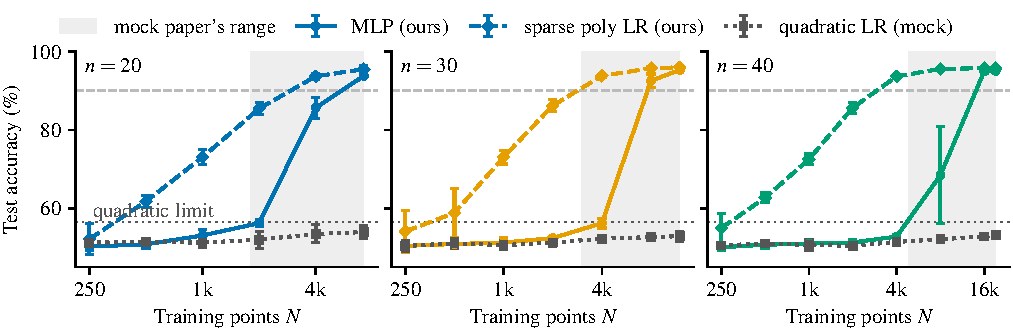
\includegraphics{fig3_learning_curves.pdf}
\vskip -0.05in
\caption{Learning curves: test accuracy against the number of training points (log scale), mean and 95\% CI over 5 splits with fixed validation and test sets; line style marks the model and colour the dataset. Grey band: the range studied by the mock paper (25--100\% of the training split). Dotted: the infinite-data limit of quadratic logistic regression (Proposition~\ref{prop:quad}). Dashed: the 90\% target.}
\label{fig:curves}
\vskip -0.15in
\end{figure*}

%=======================================================================================================
\csection{Experimental Design}
\label{sec:design}
%=======================================================================================================
We test four hypotheses against the mock paper's claims.
\textbf{H1} (approximation vs.\ estimation): the mock paper's polynomial model fails through sample complexity, not expressiveness, so the same model on coordinates selected from training data reaches $\ge90\%$ from degree 6.
\textbf{H2} (feature learning): learners that adapt their representation (an MLP, feature selection) reach $\ge90\%$ for every $n$; kernels, $k$-NN and greedy trees stay near the degree-2 ceiling.
\textbf{H3} (data): capable models improve steeply with $N$ and cross 90\% within the released data, while quadratic logistic regression plateaus at its population limit.
\textbf{H4} (adaptation): LoRA adapts KryptoNet-40 to $\ge90\%$ with few trainable parameters, while zero-shot use and frozen-representation probes are at chance.

\textbf{Validity.} (1) \emph{Shared repeated splits}: every model on Kryptonite-$n$ uses the same five stratified 60/20/20 train/validation/test splits (seeds 0--4), so comparisons are paired; Adapt uses five 64/16/20 splits with 800 test points, as in the mock paper. We report the mean and a 95\% Student-$t$ interval over splits. (2) \emph{No test leakage}: feature selection, hyper-parameters, regularisation and early stopping use only training and validation data, and each test set is used once per model and split. (3) \emph{Reproduction and controls}: we reproduce the mock paper's numbers with its code and split (e.g.\ 58.4\% for $n=20$ at degree 10), change one factor at a time, and include zero-shot use, probes, training from scratch and full fine-tuning as controls for KryptoNet-40. (4) \emph{Sampling error}: a 95\% binomial interval on 800 test points is $\pm3.5$ points.

\textbf{Feature selection.} Greedy forward selection starts from the coordinate pair whose bits give a lookup table with the lowest validation log-loss (single bits carry no signal), adds one coordinate at a time, and stops when the validation log-loss stops decreasing. A lookup table on the selected bits is the plug-in Bayes classifier and equals a full-degree polynomial in them.

\textbf{Models.} Our MLP has width 512, with depth $\in\{2,3\}$ and dropout $\in\{0,0.2\}$ chosen on validation data; it is trained by Eq.~\eqref{eq:adam} with $\alpha=10^{-3}$, $\lambda=0$, batches of 128 and early stopping on validation accuracy (patience 30, at most 300 epochs). KryptoNet-40 methods use batches of 64 and choose $\alpha\in\{3\cdot10^{-4},10^{-3},3\cdot10^{-3}\}$ on validation data. Baselines are listed in Appendix~\ref{app:details}.


%=======================================================================================================
\csection{Experimental Results}
\label{sec:results}
%=======================================================================================================
\csubsection{Anatomy of Kryptonite-n}
\label{sec:anatomy}
Every feature is a noisy bit, $x_i=b_i+\varepsilon_i$ with $\varepsilon_i\sim\mathcal N(0,0.1^2)$ and $|x_i|>0.49$, so $\bb=\sgn(\bx)$ is exact; no single bit correlates with the label. Greedy selection finds exactly 10 coordinates for every $n$, the same 10 on all five splits (Figure~\ref{fig:anatomy}). On them, Kryptonite-20/30/40 and the function computed by KryptoNet-40 (queried with synthetic inputs) share one label function up to relabelling coordinates: their majority-vote truth tables agree on 99.7--100\% of the $2^{10}$ patterns. Its Fourier coefficients take only the values $\pm\frac{9}{64},\pm\frac{3}{64},\pm\frac{1}{64}$ and $0$, and it factorises as
\begin{equation}
f(\bb)=b_p\,b_q\,h_A(\bb_A)\,h_B(\bb_B),\qquad |A|=|B|=4,
\label{eq:structure}
\end{equation}
a parity of two bits XOR-ed with two 4-bit ``gadgets'' (Appendix~\ref{app:generator}). Labels disagree with $f$ at rate $\eta=\etaPct\%$, so the Bayes accuracy is \BayesPct\%. Equation~\eqref{eq:structure} explains the difficulty: $W^{\le1}[f]=0$, $W^{\le2}[f]=(\frac9{64})^2\approx0.02$ from the single pair $P=\{p,q\}$, and \WeightFourEight\% of the weight lies at degrees 4--8. A linear program shows that $f$ is a PTF of degree 6 but not 5. Its Fourier support is a staircase of leap 2: first $P$, then $P\cup\{l\}$ for every gadget bit $l$, all with $|\hat f|\ge\frac3{64}$. Finally, KryptoNet-40 scores \SwapZeroShotPct\% on Adapt once coordinate 19 is copied into slot 0 (\ZeroShotAllPct\% without), confirming the premise of Proposition~\ref{prop:adapt}.

\begin{figure*}[t]
\centering
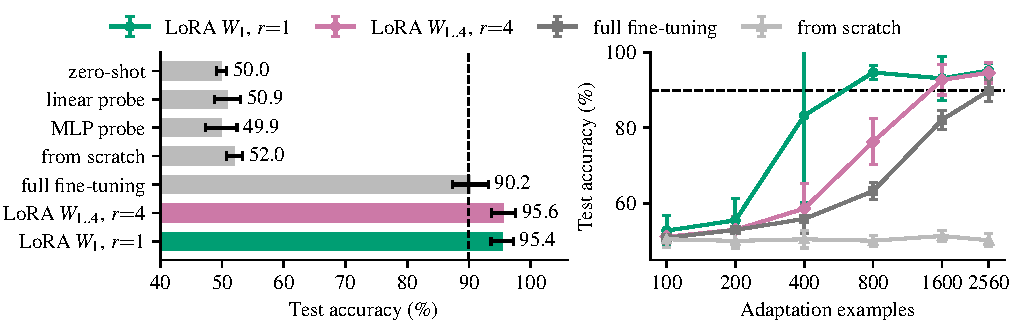
\includegraphics{fig4_kryptonet.pdf}
\vskip -0.05in
\caption{Adapting KryptoNet-40 to Kryptonite-40-Adapt. \emph{Left:} test accuracy (mean and 95\% CI over 5 splits of 800 test points) of the frozen-representation methods, the same architecture trained from scratch, full fine-tuning (809,473 trainable parameters), LoRA on $\W_1$--$\W_4$ with $r=4$ (14,496) and LoRA on $\W_1$ with $r=1$ (552). \emph{Right:} test accuracy against the number of adaptation examples. Dashed: the 90\% target.}
\label{fig:kryptonet}
\vskip -0.15in
\end{figure*}

\csubsection{Polynomial Models: Estimation, Not Approximation}
\label{sec:poly}
Our reproduction of the mock paper's model on all $n$ bits matches its Figure~1, ending at \MockTwentyTen\%, \MockThirtyTen\% and \MockFortyTen\% for $n=20,30,40$ at degree 10 (Figure~\ref{fig:poly}). Changing only the input to the 10 selected coordinates lifts the same model, with the same $C=0.85$, to \SelFixedTwenty\%, \SelFixedThirty\% and \SelFixedForty\%. The remaining gap is the regulariser: the normalised kernel gives high-degree parities tiny feature scales, which $C=0.85$ shrinks heavily. With $C$ chosen on validation data, accuracy jumps between degrees 5 and 6, exactly at the PTF degree of $f$, and reaches \SelTunedTwenty\%, \SelTunedThirty\% and \SelTunedForty\% at degree 10. The infinite-data limit agrees: degree 6 suffices (\LimitSix\%, and \LimitSeven\% from degree 7; regularised fits can slightly exceed it, as log-loss is not accuracy), degree 2 is capped at \LimitTwo\% (Proposition~\ref{prop:quad}), and the all-bit models stay near that cap at every nominal degree, as kernel theory predicts for $\log N/\log n<3$. \textbf{H1 is supported}: Kryptonite does not contradict universal approximation; its difficulty for kernels lies in the $n-10$ distractor coordinates.


\csubsection{Which Learners Succeed}
\label{sec:compare}
Table~\ref{tab:models} compares nine learners on identical splits. All learners with a fixed representation score between 50\% and 59\%: linear logistic regression is at chance because $W^{=1}[f]=0$; the quadratic and degree-10 polynomial models, $k$-NN and the RBF-kernel SVM sit near the degree-2 ceiling; and the tree ensembles reach only 52--57\% because greedy splits receive no marginal signal. The two learners that adapt their representation clear the target for every $n$: our MLP on all $n$ raw inputs, without feature engineering, reaches \MLPTwentyMean\%, \MLPThirtyMean\% and \MLPFortyMean\%, and sparse polynomial logistic regression reaches \SparseTwentyMean\%, \SparseThirtyMean\% and \SparseFortyMean\%, close to the Bayes accuracy. \textbf{H2 is supported}.

\csubsection{More Data Helps Capable Models}
\label{sec:curves}
Figure~\ref{fig:curves} extends the mock paper's Figure~2 over two orders of magnitude and to capable models. Quadratic logistic regression approaches, but cannot exceed, its population limit of \LimitTwo\%, so its flat curve measures approximation error, not the value of data. Models that can represent $f$ improve sharply: the sparse polynomial model crosses 90\% at about \NsparseTwenty, \NsparseThirty\ and \NsparseForty\ training points for $n=20,30,40$, and the MLP at about \NmlpTwenty, \NmlpThirty\ and \NmlpForty. The MLP shows the plateau-then-jump typical of SGD on sparse parities \citep{barak2022hidden}, and its jump lies \emph{inside} the range the mock paper examined, which missed it by scaling only the quadratic model. The data it needs grows with the number of distractors (\MLPgrowth-fold from $n=20$ to 40), far more slowly than the $\binom{n+6}{6}$ features of a degree-6 kernel (41-fold). \textbf{H3 is supported}: the difficulty is not intrinsic, and the target is reached within the released data.


\csubsection{Adapting KryptoNet-40}
\label{sec:kryptonet}
Zero-shot use (\ZeroShotMean\%), the linear probe (\LPMean\%) and the MLP probe (\MLPProbeMean\%) are at chance (Figure~\ref{fig:kryptonet}; all methods in Table~\ref{tab:adapt}), as Proposition~\ref{prop:adapt}(b) predicts: a linear probe recovers $b_0$ from KryptoNet-40's last hidden layer with \ProbeBitZero\% accuracy but $b_{19}$ with only \ProbeBitNineteen\%. The mock paper's ``worse than random'' scores of 46--50\% are within the $\pm3.5$-point sampling interval around 50\%; the representation does not destroy information, it lacks one bit. Training the same architecture from scratch also stays at chance (\ScratchMean\%), so pretraining matters. Full fine-tuning reaches \FullFTMean\%, and LoRA does better with far fewer parameters: rank one on $\W_1$ alone reaches \LoRAoneMean\%, matching the analytic swap of Proposition~\ref{prop:adapt}(a) (\SwapMean\%), and every LoRA configuration we tried reaches at least \LoRAminMean\%. LoRA also recovers the mechanism: on split 0, the learned $\A\in\R^{1\times40}$ has weights $\LoRAaZero$ and $\LoRAaNineteen$ on coordinates 0 and 19 and at most $\LoRAaRest$ in absolute value elsewhere, i.e.\ it moves the input of coordinate 0 to coordinate 19. With little data (Figure~\ref{fig:kryptonet}, right), rank-1 LoRA reaches \LoRAatEightHundred\% from 800 examples, where full fine-tuning reaches \FullFTatEightHundred\%. Per training step it performs \NetRatio\ of the operations of full fine-tuning (Table~\ref{tab:ops}) while training 552 instead of 809,473 parameters. \textbf{H4 is supported}.

\textbf{Hidden-set predictions.} For Kryptonite-20/30/40 we submit sparse polynomial logistic regression refitted on all labelled data (expected \SparseTwentyMean\%, \SparseThirtyMean\% and \SparseFortyMean\%; Table~\ref{tab:models}); it agrees with an independently trained MLP on \AgreeTwenty\%, \AgreeThirty\% and \AgreeForty\% of the hidden points. For Adapt we submit the majority vote of five rank-1 LoRA models trained on different 80/20 splits, which agrees with the analytic swap on \AgreeSwap\% of the hidden points.

%=======================================================================================================
\csection{Discussion}
\label{sec:discussion}
%=======================================================================================================
\textbf{What we showed.} The mock paper's three failures have three different causes, none of them a limit of machine learning: \emph{estimation} for the polynomial models, whose hypothesis class contains the Bayes classifier from degree 6 but cannot be searched in $n$ dimensions with $10^4$ samples; \emph{approximation} for the data experiment, which scaled the one model that is provably capped at \LimitTwo\%; and the \emph{choice of adaptation} for KryptoNet-40, since no frozen representation can recover a coordinate the network ignores, while a rank-one update can.

\textbf{Limitations and further experiments.} Our description of the generator is empirical: verified on every labelled set, but the hidden labels cannot be inspected; the degree sweep of the all-bit kernel model used only the mock paper's split (degree 10: all splits, Table~\ref{tab:models}). We would have liked to test the leap-based scaling of the MLP over a wider range of $n$, and harder adaptations: in a preliminary run, LoRA on $\W_1$ with $r\le16$ could not adapt KryptoNet-40 to Kryptonite-40, where all ten relevant coordinates move at once and no single move lowers the loss---the leap phenomenon again.

\textbf{Environmental impact.} We logged the wall-clock time of every experiment and converted it to energy with the Green Algorithms model \citep{lannelongue2021green}, assuming two cores at 12\,W, 4\,GB of memory at 0.3725\,W/GB and a power usage effectiveness of 1. All experiments took \TotalHours\,h on two cores, about \TotalWh\,Wh and \TotalG\,g CO$_2$e at the 2025 average carbon intensity of the GB grid, 128.8\,g/kWh \citep{energydashboard2026review}, or \TotalGhi\,g at the 175.9\,g/kWh estimate of \citet{electricitymaps2026gb} (Table~\ref{tab:energy}). Model choice matters more than these totals: at $n=40$ one fit of the mock paper's degree-10 kernel model takes \TimeKernel\,s and $O(N^3)$ operations per Newton step, our sparse polynomial model \TimeSparse\,s with over 40 points more accuracy. Adaptation reuses the energy spent on pretraining, favouring parameter-efficient methods \citep{strubell2019energy}; rank-1 LoRA trains in seconds and stores 552 numbers per task. Cheap adaptation also eases repurposing released models for unintended uses, which releases should anticipate.

\textbf{Societal perspective.} Claims that machine learning is ``all hype'' and claims of imminent general intelligence share a failure mode, outcomes not attributed to a cause; challenge datasets serve public debate best with controls and stated uncertainty.

\bibliography{references}
\bibliographystyle{icml2021}

%=======================================================================================================
\clearpage
\appendix
\csection{Proofs}
\label{app:proofs}
%=======================================================================================================
\textbf{Proposition~\ref{prop:quad}.} Write the noisy label as $s=f(\bb)\xi$ with $\xi\in\{\pm1\}$, $P(\xi=-1)=\eta$, independent of $\bx$. Let $\phi(\bx)$ collect the monomials of degree $\le2$ (in the bits $b_i$ or the raw features $x_i=b_i+\varepsilon_i$; for bits, $b_i^2=1$). The population loss $L(\bw)=\E[\log(1+e^{-s\,\bw^\top\phi(\bx)})]$ is strictly convex because $\E[\phi\phi^\top]\succ0$, so it has a unique minimiser $\bw^\star$. Negating coordinate $q$, $(b_q,\varepsilon_q)\mapsto(-b_q,-\varepsilon_q)$, leaves the distribution of $\bx$ unchanged (the bits are uniform and the noise symmetric) and maps $s$ to $-s$, because $f=b_pb_q\,g$ and $g$ does not involve $b_q$. A monomial is unchanged by this map if its degree in $x_q$ is even and negated if it is odd. Hence $L(\bw)=L(\tilde\bw)$, where $\tilde w_T=-w_T$ for monomials $T$ of even degree in $x_q$ and $\tilde w_T=w_T$ otherwise, and uniqueness forces $w^\star_T=0$ for all monomials of even degree in $x_q$. The same holds for $p$, so $\bw^\star$ is supported on monomials of odd degree in both $x_p$ and $x_q$; with degree $\le2$ the only one is $x_px_q$. The resulting classifier is $\sgn(c^\star x_px_q)=\sgn(c^\star)\,b_pb_q$, which agrees with $s=b_pb_q\,g\,\xi$ exactly when $g\xi=\sgn(c^\star)$. This has probability $\frac12(1+|\E g|)(1-2\eta)+\eta$ since $\sgn(c^\star)=\sgn(\E g)$, and $\E g=\E[f\chi_P]=\hat f(P)$. For Kryptonite, $|\hat f(P)|=\frac9{64}$ and $\eta=\etaPct\%$ give \LimitTwo\%.

\textbf{Proposition~\ref{prop:adapt}.} (a) $\W_1\Pi$ is $\W_1$ with columns 0 and 19 exchanged, so the edited network computes the pretrained network on $\Pi\bx$, and $\W_1\Pi-\W_1=-\W_1(\mathbf e_0-\mathbf e_{19})(\mathbf e_0-\mathbf e_{19})^\top=(\bw_{19}-\bw_0)(\mathbf e_0-\mathbf e_{19})^\top$ has rank one. (b) Given $(\mathbf h,z)$, $b_{19}$ is still uniform, so $P(s=1\mid\mathbf h,z)=\frac12$, $s$ is independent of $\mathbf h$, and any classifier of $\mathbf h$ is correct with probability $\frac12$.

%=======================================================================================================
\csection{The Kryptonite-3.0 Generator}
\label{app:generator}
%=======================================================================================================
For KryptoNet-40's pretraining task the parity pair is $P=\{0,10\}$ and the gadget blocks are $A=\{3,6,17,37\}$ and $B=\{8,13,26,38\}$; Adapt replaces coordinate 0 by 19, and Kryptonite-20/30/40 use the relabellings printed in notebook~01. Each gadget is a 4-bit function equal to $+1$ on 5 of its 16 inputs (up to a global sign), with 6 Fourier coefficients of magnitude $\frac38$ and 10 of magnitude $\frac18$; products with the parity give the 36, 120 and 100 coefficients of $f$ of magnitude $\frac9{64}$, $\frac3{64}$ and $\frac1{64}$. Within each block, two bits have influence $\frac58$ and two have influence $\frac38$.

%=======================================================================================================
\csection{Additional Details and Results}
\label{app:details}
%=======================================================================================================
\textbf{Reproducibility.} Figure~\ref{fig:anatomy}: \texttt{notebooks/01\_dataset\_anatomy}; Figure~\ref{fig:poly}: \texttt{02\_polynomial\_models}; Table~\ref{tab:models}: \texttt{03\_model\_comparison}; Figure~\ref{fig:curves}: \texttt{04\_learning\_curves}; Figure~\ref{fig:kryptonet} and Table~\ref{tab:adapt}: \texttt{05\_kryptonet\_lora}; Table~\ref{tab:ops}: \texttt{06\_lora\_operation\_count}; hidden-set predictions: \texttt{07\_hidden\_predictions}; Table~\ref{tab:energy}: \texttt{08\_sustainability}. Shared code is in the package \texttt{krypto}; every number in this paper is generated from the notebooks' outputs by \texttt{report/make\_numbers.py}.

\textbf{Baselines.} Linear logistic regression ($C=0.85$); the mock paper's quadratic model (explicit features, SAG, $C=0.85$, 100 iterations) and degree-10 kernel model; $k$-NN with $k\in\{1,5,15,51,151\}$ chosen on validation; an RBF-kernel SVM ($C=10$, $\gamma$ set by \texttt{scale}); a random forest with 300 trees; histogram gradient boosting with 500 iterations and early stopping. Selected MLP configurations: \MLPconfigs.

\begin{table}[h]
\caption{All KryptoNet-40 adaptation methods on Kryptonite-40-Adapt: trainable parameters and test accuracy (\%), mean $\pm$ 95\% CI over 5 splits of 800 test points.}
\label{tab:adapt}
\vskip 0.05in
\begin{center}
\setlength{\tabcolsep}{4pt}
\begin{tabular}{lrr}
\toprule
Method & Parameters & Accuracy (\%) \\
\midrule
Zero-shot & 0 & 50.0 $\pm$ 0.8 \\
Linear probe (mock) & 513 & 50.9 $\pm$ 2.1 \\
MLP probe (mock) & 263,169 & 49.9 $\pm$ 2.5 \\
From scratch & 809,473 & 52.0 $\pm$ 1.3 \\
Full fine-tuning & 809,473 & \textbf{90.2 $\pm$ 2.9} \\
LoRA on $\mathbf{W}_1$, $r=1$ & 552 & \textbf{95.4 $\pm$ 1.8} \\
LoRA on $\mathbf{W}_1$, $r=2$ & 1,104 & \textbf{95.4 $\pm$ 1.5} \\
LoRA on $\mathbf{W}_1$, $r=4$ & 2,208 & \textbf{95.3 $\pm$ 1.7} \\
LoRA on $\mathbf{W}_1$, $r=8$ & 4,416 & \textbf{95.2 $\pm$ 1.6} \\
LoRA on $\mathbf{W}_{1..4}$, $r=1$ & 3,624 & \textbf{95.3 $\pm$ 1.7} \\
LoRA on $\mathbf{W}_{1..4}$, $r=4$ & 14,496 & \textbf{95.6 $\pm$ 2.0} \\
LoRA on $\mathbf{W}_{1..4}$, $r=8$ & 28,992 & \textbf{94.8 $\pm$ 1.8} \\
Analytic rank-1 swap & 0 & \textbf{95.6 $\pm$ 1.7} \\
\bottomrule
\end{tabular}

\end{center}
\end{table}

\begin{table}[h]
\caption{Wall-clock time on two CPU cores, energy and emissions of our experiments (assumptions in Section~\ref{sec:discussion}).}
\label{tab:energy}
\vskip 0.05in
\begin{center}
\setlength{\tabcolsep}{3pt}
\begin{tabular}{lrrr}
\toprule
Notebook & Time (h) & Energy (Wh) & CO$_2$e (g) \\
\midrule
01 Anatomy & 0.00 & 0.1 & 0.0 \\
02 Polynomials & 0.66 & 16.9 & 2.2 \\
03 Comparison & 1.23 & 31.4 & 4.0 \\
04 Curves & 1.42 & 36.2 & 4.7 \\
05 KryptoNet-40 & 0.84 & 21.5 & 2.8 \\
06 Op.\ counts & 0.00 & 0.0 & 0.0 \\
07 Final models & 0.11 & 2.8 & 0.4 \\
\midrule
Total & 4.27 & 108.8 & 14.0 \\
\bottomrule
\end{tabular}

\end{center}
\end{table}

\end{document}
